\documentclass[letterpaper]{article}
\usepackage[T1]{fontenc}
\usepackage[utf8]{inputenc}
\usepackage{tocloft,siunitx,amssymb,amsmath,graphicx}
\usepackage[top=3cm,left=3cm,right=3cm]{geometry}
\usepackage{float,pgf,pgfplots}
\usepackage[american]{circuitikz}
\graphicspath{{img/}}
\renewcommand\cftsecfont{\normalfont}
\renewcommand\cftsecpagefont{\normalfont}
\renewcommand{\cftsecleader}{\cftdotfill{\cftsecdotsep}}
\renewcommand\cftsecdotsep{\cftdot}
\renewcommand\cftsubsecdotsep{\cftdot}
\renewcommand\cftsubsubsecdotsep{\cftdot}
\title{Lab :}
\author{
    Sebastián Nava López\\
    \and
    Ericka Sabrina Pensamiento R.\\
    \and
    Salvador Palos Gil
}
%\captionsetup[subfigure]{justification=raggedright}
\begin{document}
\begin{titlepage}
    \centering
    {\Huge Instituto Politécnico Nacional}\\[3ex]
    {\huge Escuela Superior de Cómputo}\\[8ex]
    {\huge Fundamental Circuit Analysis}\\[12ex]
    {\Large Lab 5: Mesh Analysis(DC)}\\[20ex]
    {\Large Group: 1CV5 Team: 7 \\[8ex]
    Sebastian Nava López\\[4ex]
    Sabrina Erika Pensamiento Robledo\\[4ex]
    Salvador Palos Gil\\[18ex]
    }
    \large{Elaboration:April 17,2018 \hspace{8em} Due date:April 24,2018}
\end{titlepage}
\tableofcontents
\newpage
\section{Introduction}
Mesh analysis (or the mesh current method) is a method that is used to solve planar circuits for the currents 
(and indirectly the voltages) at any place in the electrical circuit. Planar circuits are circuits that can be 
drawn on a plane surface with no wires crossing each other. A more general technique, called loop analysis 
(with the corresponding network variables called loop currents) can be applied to any circuit, planar or not.
Mesh analysis and loop analysis both make use of Kirchhoff’s voltage law to arrive at a set 
of equations guaranteed to be solvable if the circuit has a solution. Mesh analysis is usually easier to use 
when the circuit is planar, compared to loop analysis
%Fig1
\begin{figure}[H]
\centering
\begin{circuitikz}
\draw (0,0) to [V<=$V_S$](0,2) -- (0,4)
to [I,label=$I_s$](3,4) to [R=$R_3$](6,4) -- (6,2)
to [R=$R_2$](3,2) to [R=$R_1$](0,2)
(6,2) to [L=$L_S$] (6,0)
(3,0) to [C=$\frac{1}{sc}$](3,2)
(0,0) -- (6,0);
\end{circuitikz}
\caption{Diagram of a planar circuit}
\end{figure}
Mesh analysis works by arbitrarily assigning mesh currents in the essential meshes (also referred to as independent meshes). 
An essential mesh is a loop in the circuit that does not contain any other loop. Figure
\ref{fig:int1} labels 
the essential meshes with one, two, and three.
%Fig2
\begin{figure}[H]
\centering
\begin{circuitikz}
\draw (0,0) to [V<=$V_S$](0,2) -- (0,4)
to [I,label=$I_s$](3,4) to [R=$R_3$](6,4) -- (6,2)
to [R=$R_2$](3,2) to [R=$R_1$](0,2)
(6,2) to [L=$L_S$] (6,0)
(3,0) to [C=$\frac{1}{sc}$](3,2)
(0,0) -- (6,0);
\draw{
    [red](1.4,0.8) node {$(1)$}
    [red](3,3) node {$(2)$}
    [red](4.5,0.8) node {$(3)$}
};
\end{circuitikz}
\caption{Meshes within this circuit}
\label{fig:int1}
\end{figure}
A mesh current is a current that loops around the essential mesh and the equations are set solved in terms 
of them. A mesh current may not correspond to any physically flowing current, but the physical currents are 
easily found from them. It is usual practice to have all the mesh currents loop in the same direction. 
This helps prevent errors when writing out the equations. The convention is to have all the mesh currents looping 
in a clockwise direction. Figure \ref{fig:int2} shows the same circuit from figure \ref{fig:int1} with the mesh currents 
labeled.
%Fig3
\begin{figure}[H]
\centering
\begin{circuitikz}
\draw (0,0) to [V<=$V_S$](0,2) -- (0,4)
to [I,label=$I_s$](3,4) to [R=$R_3$](6,4) -- (6,2)
to [R=$R_2$](3,2) to [R=$R_1$](0,2)
(6,2) to [L=$L_S$] (6,0)
(3,0) to [C=$\frac{1}{sc}$](3,2)
(0,0) -- (6,0);
\draw [thick,red,->](1.35,0.8) +(80:1.6em) arc(80:-260:1.6em);
\draw [thick,red,->](4.5,0.8) +(80:1.6em) arc(80:-260:1.6em);
\draw [thick,red,->](3,3) +(80:1.6em) arc(80:-260:1.6em);
\draw{
    [red](1.4,0.8) node {$I_1$}
    [red](3,3) node {$I_2$}
    [red](4.5,0.8) node {$I_3$}
};
\end{circuitikz}
\caption{Labeled mesh currents}
\label{fig:int2}
\end{figure}
Solving for mesh currents instead of directly applying Kirchhoff's current law and Kirchhoff's voltage law can 
greatly reduce the amount of calculation required. This is because there are fewer mesh currents than there are physical 
branch currents. In figure \ref{fig:int2} for example, there are six branch currents but only three mesh
currents.\\[1ex]
{\large\textbf{Setting up the equations}}\\[2ex]
Each mesh produces one equation. These equations are the sum of the voltage drops in a complete loop of 
the mesh current. For problems more general than those including current and voltage sources, the voltage drops will 
be the impedance of the electronic component multiplied by the mesh current in that loop.

If a voltage source is present within the mesh loop, the voltage at the source is either added or 
subtracted depending on if it is a voltage drop or a voltage rise in the direction of the mesh current.
For a current source that is not contained between two meshes, the mesh current will take the positive 
or negative value of the current source depending on if the mesh current is in the same or opposite direction 
of the current source. The following is the same circuit from above with the equations needed to solve for 
all the currents in the circuit.
\[
    \begin{cases}
        Mesh\ 1:I_1=I_s=0\\
        Mesh\ 2:-V_s+R_1(I_2-I_1)+\frac{1}{sC}(I_2-I_3)=0\\
        Mesh\ 3:\frac{1}{sC}(I_3-I_2)+R_2(I_3-I_1)+L_sI_3=0
    \end{cases}
    \]
Once the equations are found, the system of linear equations can be solved by using any technique to
solve linear equations.\\[1ex]
{\large\textbf{Special cases}}\\[2ex]
%Fig4
\begin{figure}[H]
\centering
\begin{circuitikz}
\draw (0,0) to [V<=$V_S$](0,2)
to[R=$R_1$](3,2)
to[R=$R_2$](6,2) -- (6,0) -- (0,0)
(3,0) to [I,label=$I_S$](3,2);
\draw [thick,red,->](1.35,0.8) +(80:1.6em) arc(80:-260:1.6em);
\draw [thick,red,->](4.5,0.8) +(80:1.6em) arc(80:-260:1.6em);
\draw{
    [red](1.35,0.8) node {$I_1$}
    [red](4.5,0.8) node {$I_2$}
};
\end{circuitikz}
    \caption{Circuit with a current source affecting both meshes}
\end{figure}
Supermesh

A supermesh occurs when a current source is contained between two essential meshes. The circuit is first treated as 
if the current source is not there. This leads to one equation that incorporates two mesh currents. Once 
this equation is formed, an equation is needed that relates the two mesh currents with the current source. 
This will be an equation where the current source is equal to one of the mesh currents minus the other. The 
following is a simple example of dealing with a supermesh.
\[
    \begin{cases}
        Mesh\ 1,2: -V_s+R_1I_1+R_2I_2=0\\
        Dependent\ Variable:I_s=I_2-I_1
    \end{cases}
    \]
Dependent sources

A dependent source is a current source or voltage source that depends on the voltage or current of another element 
in the circuit. When a dependent source is contained within an essential mesh, the dependent source should be 
treated like an independent source.
%Fig5
\begin{figure}[H]
\centering
\begin{circuitikz}
\draw (0,0) to [V<=$V_S$](0,2)
to[R=$R_1$](3,2)
to[R=$R_2$](6,2) 
to [cV,label=$3\cdot I_x$](6,0) -- (0,0)
(3,0) to [R=$R_3$,i_<=$I_x$](3,2);
\draw [thick,red,->](1.35,0.8) +(80:1.6em) arc(80:-260:1.6em);
\draw [thick,red,->](4.5,0.8) +(80:1.6em) arc(80:-260:1.6em);
\draw{
    [red](1.35,0.8) node {$I_1$}
    [red](4.5,0.8) node {$I_2$}
};
\end{circuitikz}
    \caption{Circuit containing a variable voltage source}
\end{figure}
After the mesh equation is formed, a dependent source equation is needed. This equation is generally called a 
constraint equation. This is an equation that relates the dependent source’s variable to the voltage or 
current that the source depends on in the circuit. The following is a simple example of a dependent source.
\[
    \begin{cases}
        Mesh\ 1: -V_s+R_1I_1+R_3(I_1-I_2)=0\\
        Mesh\ 2:R_2I_2+3I_x+R_3(I_2-I_1)=0\\
        Dependent\ Variable:I_x=I_1-I_2
    \end{cases}
    \]
\newpage
\section{Development}
\subsection{Verification of mesh analysis in DC}
Using a circuit as the one shown in figure \ref{fig:diag1}: 
\begin{figure}[H]
    \centering
\begin{circuitikz}
    \draw
        (0,2) to [V](0,0)
        (0,2) -- (0,4)
        (0,4) to [R=$\SI{680}{\ohm}(R_1)$](3,4)
        to [V](6,4) to
        (6,2) to [R,*-](3,2)
        to [R,*-*](0,2)
        (6,2) to [R=$\SI{1}{\kilo\ohm}(R_5)$](6,0) -- (0,0)
        (3,0) to [R=$\SI{470}{\ohm}(R_4)$,*-](3,2)
        {
            [anchor = south east](5.4,2.2) node {$\SI{560}{\ohm}(R_3)$}
            [anchor = south east](2.4,2.2) node {$\SI{1}{\kilo\ohm}(R_2)$}
            [anchor = south east](0,1.4) node {$\SI{9}{\volt}(V_{S1})$}
            [anchor = south east](5.4,4.4) node {$\SI{5}{\volt}(V_{S2})$}
        }
        ;
\end{circuitikz}
    \caption{Circuit diagram}
    \label{fig:diag1}
\end{figure}
we measured current in each mesh ,and voltage values in each resistance.
\subsubsection{Calculations}
Using mesh analysis to calculate currents, we assign the direction of all currents clockwise, as
shown in figure \ref{fig:diag2}:
\begin{figure}[H]
    \centering
    \begin{circuitikz}
        \draw
        (0,2) to [V](0,0)
        (0,2) -- (0,4)
        (0,4) to [R=$R_1$](3,4)
        to [short,i_=$I_1$](3.5,4)
        to [V](6,4) to
        (6,2) to [R,*-](3,2)
        to [R,*-*](0,2)
        (6,2) to [R=$R_5$](6,0) -- (0,0)
        (3,0) to [R=$R_4$,*-](3,2)
        (3,0) to [short,i_=$I_2$](0,0)
        (6,0) to [short,i_=$I_3$](3,0)
        {
            [anchor = south east](5.4,2.2) node {$R_3$}
            [anchor = south east](2.4,2.2) node {$R_2$}
            [anchor = south east](0,1.4) node {$V_{S1}$}
            [anchor = south east](5.4,4.4) node {$V_{S2}$}
            [anchor = south east](1.8,0.7) node {$(2)$}
            [anchor = south east](4.9,0.7) node {$(3)$}
            [anchor = south east](3.4,2.7) node {$(1)$}
        }
        ;
    \end{circuitikz}
    \caption{Circuit diagram with proposed current directions}
    \label{fig:diag2}
\end{figure}
Applying Kirchhoff's Current Law(KCL) in mesh 1 according to figure \ref{fig:diag2}:
\begin{gather*}
    V_{R3}+V_{R2}+V_{R1}+V_{S2} = 0\\
    560(I_1-I_3)+1000(I_1-I_2)+680I_1+5 = 0
\end{gather*}\\[-6.5ex]
\begin{equation}2240I_1-1000I_2-560I_3 = -5\label{eq:1}\end{equation}
    in mesh 2:
\begin{gather*}
    -V_{S1}+V_{R2}+V_{R4} = 0\\
    -9+1000(I_2-I_1)+470(I_2-I_3) = 0
\end{gather*}\\[-6.5ex]
\begin{equation}-1000I_1+1470I_2-470I_3 = 5\label{eq:2}\end{equation}
    in mesh 3:
\begin{gather*}
    V_{R4}+V_{R3}+V_{R5} = 0\\
    470(I_3-I_2)+560(I_3-I_1)+100I_3 = 0
\end{gather*}\\[-6.5ex]
\begin{equation}-560I_1-470I_2-2030I_3 = 0\label{eq:3}\end{equation}
    therefore we have the following linear equation system:
    \[
        \begin{bmatrix}
            2240 & -1000 & -1560\\
            -1000 & 1470 & -470\\
            -560 & -470 & 2030
        \end{bmatrix}
    \begin{bmatrix}
        -5\\
        9\\
        0
    \end{bmatrix}
    =
    \begin{bmatrix}
        I_1\\
        I_2\\
        I_3
    \end{bmatrix}
\]
To solve the system using Crammer's rule we need to compute the required determinants($\Delta$). For
$\Delta$ we have that:
    \begin{gather*}
        \Delta = det\Bigg(
        \begin{bmatrix}
            2240 & -1000 & -560\\
            -1000 & 1470 & -470\\
            -560 & -470 & 2030
        \end{bmatrix}
        \Bigg)\\
        \Delta = 2240\cdot det\bigg(
        \begin{bmatrix}
            1470 & -470\\
            -470 & 2030
        \end{bmatrix}
        \bigg)
        +1000\cdot det\bigg(
        \begin{bmatrix}
            -1000 & -470\\
            -560 & 2030
        \end{bmatrix}
        \bigg)
        -560\cdot det\bigg(
        \begin{bmatrix}
            -1000 & 1470\\
            -560 & -470
        \end{bmatrix}
        \bigg)\\
        \Delta = 2240\cdot(2763200)+1000\cdot(-2293200)-560\cdot(1293200)\\
        \therefore\Delta = 3172200000
    \end{gather*}
$\Delta_1$ is given by:
    \begin{gather*}
        \Delta_1 = det\Bigg(
        \begin{bmatrix}
            -5 & -1000 & -560\\
            9 & 1470 & -470\\
            0 & -470 & 2030
        \end{bmatrix}
        \Bigg)\\
        \Delta_1 = -5\cdot det\bigg(
        \begin{bmatrix}
            1470 & -470\\
            -470 & 2030
        \end{bmatrix}
        \bigg)
        +1000\cdot det\bigg(
        \begin{bmatrix}
            9 & -470\\
            0 & 2030
        \end{bmatrix}
        \bigg)
        -560\cdot det\bigg(
        \begin{bmatrix}
            9 & 1470\\
            0 & -470
        \end{bmatrix}
        \bigg)\\
        \Delta_1 = -5\cdot(2763200)+1000\cdot(18270)-560\cdot(-4230)\\
        \therefore\Delta_1 = 6822800
    \end{gather*}
$\Delta_2$ is given by:
    \begin{gather*}
        \Delta_2 = det\Bigg(
        \begin{bmatrix}
            2240 & -5 & -560\\
            -1000 & 9 & -470\\
            -560 & 0 & 2030
        \end{bmatrix}
        \Bigg)\\
        \Delta_2 = 2240\cdot det\bigg(
        \begin{bmatrix}
            9 & -470\\
            0 & 2030
        \end{bmatrix}
        \bigg)
        +5\cdot det\bigg(
        \begin{bmatrix}
            -1000 & -470\\
            -560 & 2030
        \end{bmatrix}
        \bigg)
        -560\cdot det\bigg(
        \begin{bmatrix}
            -1000 & 9\\
            -560 & 0
        \end{bmatrix}
        \bigg)\\
        \Delta_2 = 2240\cdot(18270)+5\cdot(-2293200)-560\cdot(5040)\\
        \therefore\Delta_2 = 26636400
    \end{gather*}
$\Delta_3$ is given by:
    \begin{gather*}
        \Delta_3 = det\Bigg(
        \begin{bmatrix}
            2240 & -1000 & -5\\
            -1000 & 1470 & 9\\
            -560 & -470 & 0
        \end{bmatrix}
        \Bigg)\\
        \Delta_3 = 2240\cdot det\bigg(
        \begin{bmatrix}
            1470 & 9\\
            -470 & 0 
        \end{bmatrix}
        \bigg)
        +1000\cdot det\bigg(
        \begin{bmatrix}
            -1000 & 9\\
            -560 & 0
        \end{bmatrix}
        \bigg)
        -5\cdot det\bigg(
        \begin{bmatrix}
            -1000 & 1470\\
            -560 & -470
        \end{bmatrix}
        \bigg)\\
        \Delta_3 = 2240\cdot(4230)+1000\cdot(5040)-5\cdot(1293200)\\
        \therefore\Delta_3 = 16281200
    \end{gather*}
Finally:
\begin{gather*}
I_1 = \frac{\Delta_1}{\Delta} = \frac{6822800}{3172200000}\qquad\therefore I_1 =
\SI{2.151}{\milli\ampere}\\
I_2 = \frac{\Delta_2}{\Delta} = \frac{26636400}{3172200000}\qquad\therefore I_2 =
\SI{8.397}{\milli\ampere}\\
I_3 = \frac{\Delta_3}{\Delta} = \frac{8049200}{3172200000}\qquad\therefore I_3 =
\SI{2.537}{\milli\ampere}\\
\end{gather*}
Now that we have values for all the currents, voltage values in each resistor are given as follows:
Voltage in $R_1$:
\begin{gather*}V_{R1} = R_1\cdot I_1
    =(\SI{680}{\ohm})(\SI{2.151}{\milli\ampere})\qquad\therefore V_{R1} =
\SI{1.463}{\volt}
\end{gather*}
Voltage in $R_2$:
\begin{gather*}V_{R2} = R_2\cdot(I_2-I_1)
    =(\SI{1}{\kilo\ohm})(\SI{8.397}{\milli\ampere}-\SI{2.151}{\milli\ampere})\qquad\therefore V_{R2} =
\SI{6.246}{\volt}
\end{gather*}
Voltage in $R_3$:
\begin{gather*}V_{R3} = R_3\cdot(I_3-I_1)
    =(\SI{560}{\ohm})(\SI{2.537}{\milli\ampere}-\SI{2.151}{\milli\ampere})\qquad\therefore V_{R3} =
\SI{0.216}{\volt}
\end{gather*}
Voltage in $R_4$:
\begin{gather*}V_{R4} = R_4\cdot(I_2-I_3)
    =(\SI{470}{\ohm})(\SI{8.397}{\milli\ampere}-\SI{2.537}{\milli\ampere})\qquad\therefore V_{R4} =
\SI{2.754}{\volt}
\end{gather*}
Voltage in $R_5$:
\begin{gather*}V_{R5} = R_5\cdot I_3
    =(\SI{1}{\kilo\ohm})(\SI{2.537}{\milli\ampere})\qquad\therefore V_{R5} =
\SI{2.537}{\volt}
\end{gather*}
\subsubsection{Simulation}
\begin{figure}[H]
    \centering
    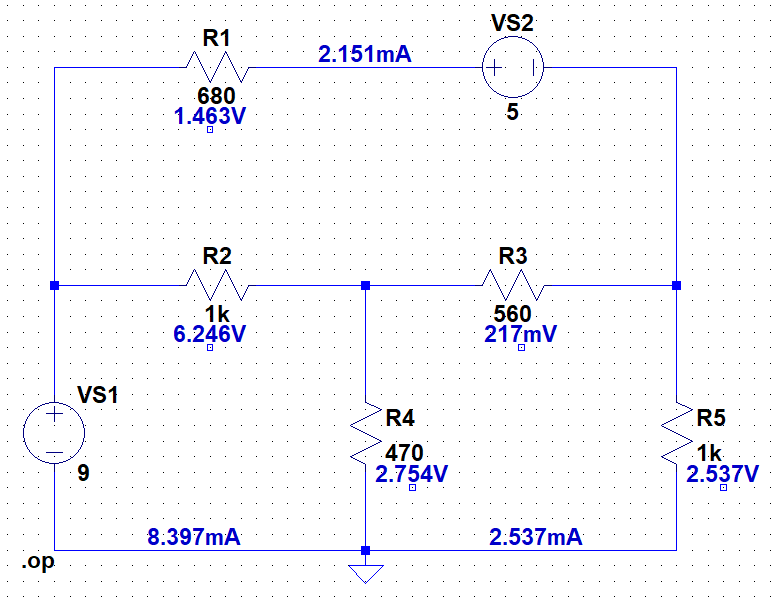
\includegraphics[width=.65\linewidth]{sim1}
    \caption{Circuit simulation}
\end{figure}
\subsubsection{Measurements}
\begin{figure}[H]
    \centering
    \begin{tabular}{|c|c|c|c|}\hline
        Measurements & Theoretical Value(\si{\milli\ampere}) & Measured Value(\si{\milli\ampere}) &
        Simulated Value (\si{\milli\ampere})\\\hline
        $I_{1}$ & 2.151 & 2.180 & 2.151 \\\hline
        $I_{2}$ & 8.397 & 8.460 & 8.397 \\\hline
        $I_{3}$ & 2.537 & 2.580 & 2.537 \\\hline
    \end{tabular}
    \caption{Current values measured, calculated and simulated}
\end{figure}
\begin{figure}[H]
    \centering
    \begin{tabular}{|c|c|c|c|}\hline
        Measurements & Theoretical Value(\si{\volt}) & Measured Value(\si{\volt}) &
        Simulated Value (\si{\volt})\\\hline
        $V_{R1}$ & 1.463 & 1.482 & 1.463 \\\hline 
        $V_{R2}$ & 6.246 & 6.250 & 6.246 \\\hline 
        $V_{R3}$ & 0.216 & 0.218 & 0.217 \\\hline 
        $V_{R4}$ & 2.754 & 2.783 & 2.754 \\\hline 
        $V_{R5}$ & 2.537 & 2.560 & 2.537 \\\hline 
    \end{tabular}
    \caption{Voltage values measured, calculated and simulated}
\end{figure}
\section{Questions}
\textit{\textbf{What's a mesh in an electrical circuit}}

A mesh is any closed path in an electrical circuit.\\
\textit{\textbf{Describe what the mesh analysis method in circuit theory consists of?}}

Mesh analysis (sometimes referred to as a mesh current method) is a technique used to determine the voltage 
or current of any element in a flat circuit. A flat circuit is one that can be drawn in 
a plane so that no branch is below or above any other. This technique is based on Kirchhoff'
s law of tensions. The advantage of using this technique is that it creates a system of equations to 
solve the circuit, minimizing in some cases the process to find a voltage or current in a circuit.\\
\textit{\textbf{What are the advantages of applying mesh analysis ?}}

It helps us to reduce circuits, provides the basics for all general analysis methods (connections and devices), 
help in the analysis of nodes,and mainly it helps us by giving a system of equations to then find what we 
want in the circuit.\\
\textit{\textbf{The calculated values of voltage and current in each resistor coincide with those measured.Why?}}

Yes, the calculated and measured values coincide, because the mesh analysis method helped us by giving a system of equations that predicts the behavior of the components that act on each mesh of the circuit.
\section{Conclusions}
{\large Sabrina:}\\
text%
\\[2ex]
{\large Salvador:}\\
Mesh analysis is fundamental to know how each component of the circuit interacts and to be able to predict 
what each element in the circuit will experience. In practice we used the analysis to understand that if 
the current and voltage that the elements experience is different when there are 2 voltage sources.
\\[2ex]
{\large Sebastián:}\\
We used mesh analysis to find the currents in a circuit which contains three meshes; first, we
described the voltages flowing across each mesh and, using Ohm's Law, we obtained three expressions
which had three different variables, the currents. Finally, solving the linear equations system
formed by this three, we had the current values in each mesh, with this values we determined the
currents passing in each resistor. After wiring the same circuit, we verified that our measured
currents and voltages were closer to our calculated values, thus confirming our mesh analysis
applied to our circuit.
\end{document}
